\chapter{The Blockchain And Hyperledger Fabric Background}


\section{The Blockchain} 

Blockchain[9] has become one of the most hyped technology trends. it provides a new way of managing and storing data, in addition, it provides capabilities for solving complex computing solutions. Taken further blockchain could be a cornerstone for secure data transfer and exchange on the internet.
Trust on the internet considered one of the most stubborn problems, and here blockchain came to play. unlike the traditional database that requires a central authority which authorizes the access to it and determines what is inserted and deleted. The traditional database has more two major flaws[10]. 
First, it has a single point of failure, in addition, it will have only one major central authority.\\
Central authority between many stakeholder levies additional overhead. For instance processing time and cost, vulnerability and limited participation between parties.  
Blockchain introduces a new way of storing data instead of a central server the data will be stored on every single node on the network in a distributed fashion. 

It's worth mentioning that Blockchain was based on a collection of related technologies, for instance, The public key infrastructure or PKI.
Public Key Infrastructure provides an infrastructure for digital certificate management. \\ 
PKI will add Trustworthiness of the keys, thus we can avoid a situation when Anybody could have uploaded their own keys and claimed they belong
to an email address (masquerading). After the organization generates the public and private key it will share the public key and here comes the role of a digital signature, which is equivalent of
a handwritten signature, but offering far more inherent security, a digital signature is intended to solve the problem of tampering and impersonation in digital communications. \\
Digital signatures can provide the added assurances of evidence to an origin, identity, and status of an electronic document,
transaction or message, as well as acknowledging informed consent by the signer. \\


in addition, it's also beneficial to cover some terms. 
A nonce is a number that is used once and never used again it helps to avoid duplicate transactions in digital transmission, for example, sometimes the data entered the database may have the same identifier adding nonce making it a bit harder for occasional replication. 
A Hash function is a mathematical process that takes data of any size and returns a unique hash with a fixed size no matter the size of the input data, however, it's only a one-way function thus it's hard to generate the original text from the hashed value. one major advantage of hashing is to keep the database small, as storing only the hash value save a tremendous amount of disk. in blockchain, hashes are used as an identifier for blocks and transactions. \\ 

Blockchain[11] is a distributed database and its entries are immutable in other words it's not living on one server it's distributed and the data stored in it can't be modified or deleted. 
Blockchain is a sequence of blocks, which holds a complete list of transaction records like a conventional public ledger. 
namely that the information is packaged into blocks, which link to form a chain with other blocks of similar information.
It is this act of linking blocks into a chain that makes the information stored on a blockchain so trustworthy. Once the data is recorded in a block it cannot be altered without having to change every block that came after it, making it impossible to do so without it being seen by the other participants on the network. Normally, each block contains the data it is recording, for example, transaction details as well as timestamps of when that information was recorded. It will also include a digital signature linked to the account that made the recording and a unique identifying link, in the form of a hash to the previous block in the chain. It is this link that makes it impossible for any of the information to be altered or for a block to be inserted between two existing blocks. In order to do so, all following blocks would need to be edited too. As a result, each block strengthens the previous block and the security of the entire blockchain because it means more blocks would need to be changed to tamper with any information. When combined, all of these create unquestionable storage of information, one that cannot be altered.  \\ 


In traditional database data is stored in tables, rows and, columns usually in every table the stored data is related. 
For instance, a table might contain a customer's name and address. It will also contain a unique key for every record to link one table to another.
In a client-server model, the database usually lives on a single logical server and it's queried as request and the server runs the query and sends back the result to the client. Another aspect of this is in web architecture there are usually other tiers like a client, web server and load balancer, web servers and database servers are distributed among physical servers, however, logically they are governed by the same set of rules and said to be centralized even if they are physically distributed. the traditional database is useful however it's also vulnerable.
A blockchain database is structured in a way that it comprises of specific blocks of data organized in a specific structure, However, there is a huge difference in how the database is hosted a copy of a blockchain database resides on every node participate in the network there is no central server and it's not hierarchical it's a peer to peer. For example, if a user joins a blockchain environment all the database will be downloaded to his computer next each transaction happens on the blockchain will be recorded in every instance of the blockchain database in this way it's called a distributed Ledger. 
for every transaction, consensus must be reached by all participating nodes.
Lastly, a blockchain distributed ledger is immutable entries made will never be edited once a transaction occurred it will always be there. there is no remedy. \\ 

The ledger is updated by a smart contract. A smart contract[12] is a computer code running on top of a blockchain containing a set of rules under which the parties to that smart contract agree to interact with each other. If and when the pre-defined rules are met, the agreement is automatically enforced. The smart contract code facilitates, verifies, and enforces the negotiation or performance of an agreement or transaction. It is the simplest form of decentralized automation.
 \\ 
 \hyperref[fig:bcvsdb]{Figure 2.1} depicts the main characteristics of the blockchain and the differences between the traditional databases.
\begin{figure}[H]
	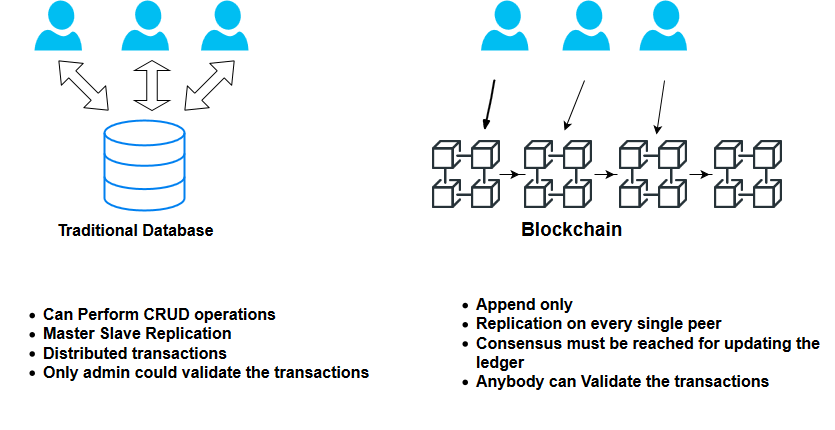
\includegraphics[width=15cm,height=10cm]{images/bcvsdb.png}
	\caption{Blockchain VS Traditional Database}
	\label{fig:bcvsdb}
	\end{figure}

\section{Hyperledger Fabric}
 
\subsection{Introduction}
Hyperledger Fabric[13] is an Open-source permissioned Blockchain platform it was profounded under the Linux Foundation. Hyperledger Fabric became one of the fastest growing projects in the Linux Foundation. 
Hyperledger Fabric is the first platform that supports developing the smart contracts("chaincode")[12] in general-purpose programming languages such as Java, Go and Node.js.
In a public or permissionless blockchain anyone can participate without a specific identity. Hypeperledger Fabric is a permissioned blockchain in a simplified way this means the participants will be known to each other instead of being anonymous and fully untrusted. 
It provides a way to secure the interactions between different parties, which they not particularly trusting each other having that it reinforces the trust between different entities.
Hypeledger Fabric is an enterprise distributed ledger based on GO programming language that uses smart contracts. 
The architecture of Fabric follows an execute-order-validate paradigm for distributed execution of untrusted code in an untrusted environment. It separates the transaction flow into three steps, which may be run on different entities in the system: (1)execute where Transactions are executed(using chaincode) in any order, possibly even in parallel. (2)ordering through a consensus protocol When peers reach an agreement on the results of a transaction, it’s added to the ledger and spread to all peers. (3) transaction validation by the peers which can check whether a later transaction was invalidated by an earlier transaction. For example, this prevents one item from being sold two times (called double-spending)[14].\\ 

Hyperledger is distributed by design there is no single point of failure or a single place that the information is stored.
All the participants are holding the same data, moreover, the data cannot be altered once it's stored, therefore Hyperledger fabric reinforces the trust among the participants.


\subsection{Hyperledger Fabric Components} 

Hyperledger Fabric comprises of three main components:
\begin{itemize}
  \item Hyperledger Fabric CA (Certificate Authority) 
  \item Hyperledger Fabric Peer 
  \item Hyperledger  Fabric Orderer 
\end{itemize} 
\bigskip
\textbf{Hyperledger Fabric CA:} every single operation on hyperledger fabric must be signed with certificates.
Fabric CA is a high-quality tool that pursues cryptographic standards to generate certificates these certificates are per user and attributes could be added while generating those certificates, therefore specific rules and permissions could be enforced per specific group of users. 
It is a place to generate certificates and where the account would be created this process called enrollment you provide username and password and the fabric CA does all the magic by the Issuance of Enrollment Certificates used for signing and identifying users identities. 
In addition, Fabric-CA could be attached to an existing LDAP and all attributes would be fetched from there. 
Fabric CA registers and enrolls the users, then it provides the certificate to SDK and the SDK signs all requests that will be executed inside Hyperledger fabric. \\ 

\textbf{Peer:} is the place where the ledger blockchain is stored there could be more than one peer especially in production they contain the same ledger.  the request is sent from the SDK to peers, in order to do operations on the ledger like insert or query.  The main role of the peer is to endorse and update the ledger. all peers are synced automatically adding more peers in the network the other peer will automatically update the state of the newly joined peer, and this is facilitating the scalability of hyperledger fabric.  \\ 

\textbf{Orderer:} is coming into the heart of the consensus algorithm its main role is to provide order of operation before anything committed to the ledger it should be first validated and verified by the order and orderer creates the blocks so all transactions are stored into blocks and once blocks are full it will be sent to peers to be committed into the ledger. namely, the orderer is responsible for determining the order of operations.
There are several different implementations of ordering the first type is Solo which is mainly for development and this is only one instance if this instance fails all the operations for updating the ledger will fail, and the second type is Kafka which is a Crash fault tolerance (CFT) implementation is suitable for the production environments.\\

It's also worth mentioning \textbf{the channel} concept channels are a method developed in hyperledger fabric for data isolation More broadly it's a completely isolated instance of hyperledger fabric. every channel is completely independent and they never exchange data. when building network peers must be a part of the channel when creating peers, the peers should join a channel. with channel concept, the privacy and confidentiality of the data will be assured. the channel should be created and configured by a specific tool from hyper ledger fabric. in addition, one peer could be a part of different channels.  \\
 

\textbf{Chaincode} is a smart contract which is a program that reads and updates the ledger data, usually, all the business logic is written inside the chaincode. namely, the only way of interacting with the ledger will be only via the chaincode. 
The chaincode could be written in general purpose programming languages like Go, Java, and Javascript. The chaincode could adapt to any desired complex business logic. \\

One important note that the chaincode must be apart of a channel inside one channel there could be as many as chaincodes. it could be possible to define all the business logic on one chaincode or split it amongst many chaincodes. 
The chaincode has to be installed and later instantiated. when writing chaincode it must be installed on every single peer that is a part of that channel this could be done using SDK or by using the peer itself. \\
 
Installing the chaincode on the peers is a must once it's the only way to interact with the ledger which resides on the peers. 
Once the chaincode is installed it should be then instantiated. 
Instantiating the chaincode will start a container that runs the chaincode while instantiating the chaincode the endorsement policy would be applied which will be responsible for validating and matching the rule on every single operation. For instance, applying a rule in a way  that for every transaction every peer must agree on adding the record otherwise the transaction will be rejected. \\
 
\textbf{Memebership Service Provider MSP}: is one of the most fundamental concepts of hyperledger fabric is a setup of cryptographical materials where the organizations will be defined. every single on hyperledger fabric must have its cryptographic certificates that define if a specific node belongs to specific organization generating the cryptographic material is trivial by hyperledger fabric tool cryptogen. 
The most essential part is that only peers that are part of the same MSP could communicate with each other. other peers couldn't the peer must be a part of the organization and this is defined by the peer's certificate later when configuring the channel all the public certificates will be shared on the configuration thus only the configured peer with a shared certificate could communicate and be a part of this channel. \\

\textbf{The State Database:} In the blockchain concept, the state of the data would be tracked from the transactions history, for instance, assume that there is a simple balance transfer network. Person A sends 100 euros to person B and person C sends another 100 euros to person C. the current balance of person B should be 200 euros, however The blockchain consisted of serious of transactions, in order to calculate the latest state of the accounts all transactions history should be reviewed and validated. For more efficient way Hyperledger fabric uses a key-value store database to update the latest state of the data in an efficient way.
Chaincode invocations execute transactions against the current state data. To make these chaincode interactions extremely efficient, the latest values of all keys are stored in a state database. The state database is simply an indexed view into the chain of transactions log, it can, therefore, be regenerated from the chain at any time. The state database will automatically get recovered (or generated if needed) upon peer startup before transactions are accepted.\\

\textbf{World state} or state database are options include LevelDB and CouchDB. LevelDB is the default state database embedded in the peer process and stores chaincode data as key-value pairs. CouchDB is an optional alternative external state database that provides addition query support when your chaincode data is modeled as JSON, permitting rich queries of the JSON content. Leveraging CouchDB as Hyperledger fabric state database[15].


\cleardoublepage

\subsection{Under The hood Hyperledger Fabric }

In this part, we will try to explain how hyperledger fabric works under the hood,
Assume that a user  wanted to exchange the ownership of some assets, and The client wants to make a transaction. 
The first step is that the user has to register and enroll in the organization using Fabric CA and get back the proper cryptographic materials that authorize him to interact with the network. Then the SDK will be responsible for preparing the transaction as a transaction proposal. 
The transaction proposal will be sent to one or more peers. At this point the peer accepts this proposal and simulates it, the result of this simulation will be called read and write sets. The read set contains a list of unique keys and their committed versions that the transaction reads during the simulation. The write set contains a list of unique keys and their new values that the transaction writes. At this phase, the ledger is not updated and the assets values remaining the same. 
The endorsing peers which are special kind of peers that its role is to verify and approve the transaction. this is will be done by validating the format and the signature of the transaction, and if the application user is authorized to make this transaction. 
Then the peers are sending back those transaction responses to the SDK. The SDK collects all these transaction responses and signs it and sends it to the orderer, the orderer node verifies the transaction signature and the endorsement policy. no matter if the transaction approved or rejected it will be stored on the blockchain, however, the state of the ledger will not be updated in case of the failure. Once the orderer node receives the transaction responses from the SDK, it will verify the read and write sets collected from every single peer and assuring that all transaction responses are the same. 
Finally, in case the transaction is valid the orderer will send the transaction to the committing peers to be committed and updating the ledger.
\hyperref[fig:transactionflow]{Figure 2.2} depicts Hyperledger fabric transaction flow [1]. 
\begin{figure}[H]
	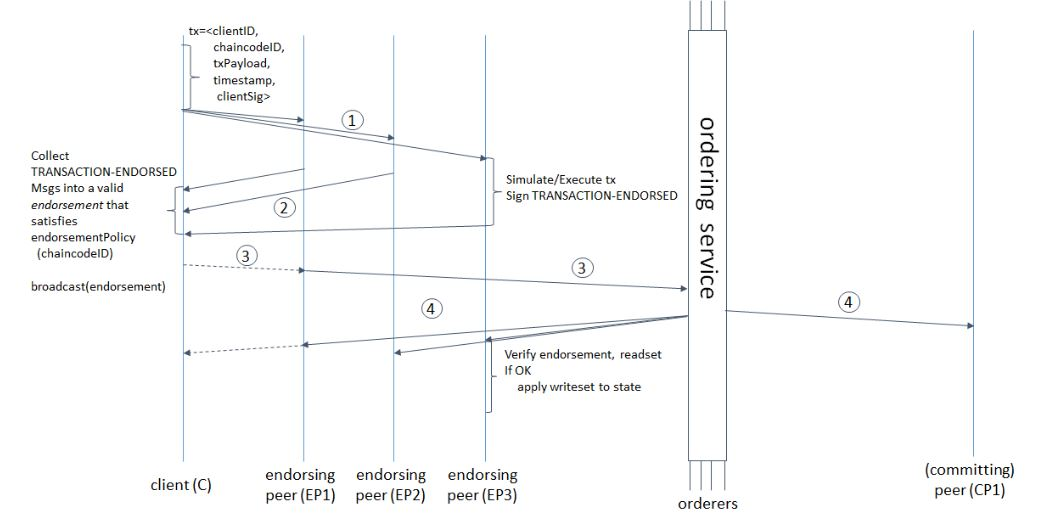
\includegraphics[width=15cm,height=10cm]{images/transactionflow.jpg}
	\caption{Hyperledger Fabric Transaction Flow Diagram}
	\label{fig:transactionflow}
	\end{figure}

 
 

 
 

 
 





 



 
  